\documentclass[9pt,aspectratio=169]{beamer}
\usepackage[utf8]{inputenc}
\usepackage[english,russian]{babel}
\usetheme{default}
\usepackage{color}
\setbeamertemplate{navigation symbols}{}

\begin{document}

\begin{frame}

\frametitle{
\color[RGB]{153,153,153}
	\begin{flushright}
	    \textbf{{\color[RGB]{22,83,126} А}лфавит и его подмножества}\qquad\qquad\qquad
	\end{flushright}
	\hrule
	\vskip -1.5cm\hskip -0.4cm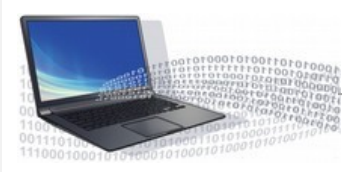
\includegraphics[scale=0.4]{logo.png}
}

%\noindent 
\color[RGB]{44,137,4}
\textbf{Алфавит}
\color{black}
– конечное множество различных знаков (букв), символов, для которых определена операция конкатенации (присоединения символа к символу или цепочке символов). \\[0.5em]

\color[RGB]{44,137,4}
\textbf{Знак (буква)}
\color{black}
– любой элемент алфавита (элемент $x$ алфавита $X$, где $x \in X$). \\[0.5em]

\color[RGB]{44,137,4}
\textbf{Слово}
\color{black}
– конечная последовательность знаков (букв) алфавита. \\[0.5em]

\color[RGB]{44,137,4}
\textbf{Словарь (словарный запас)}
\color{black}
– множество различных слов над алфавитом.

\end{frame}

\begin{frame}

\frametitle{
\color[RGB]{153,153,153}
	\begin{flushright}
		\textbf{{\color[RGB]{22,83,126} К}одирование данных}\qquad\qquad\qquad
	\end{flushright}
	\hrule
	\vskip -1.5cm\hskip -0.4cm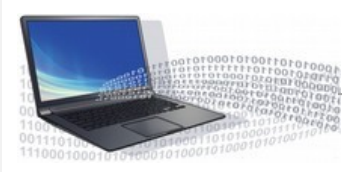
\includegraphics[scale=0.4]{logo.png}
}

\color[RGB]{44,137,4}
\textbf{Кодирование (модуляция) данных}
\color{black}
— процесс преобразования символов алфавита $X$ в символы алфавита $Y$. \\[0.5em]

\color[RGB]{44,137,4}
\textbf{Декодирование (демодуляция)}
\color{black}
— процесс, обратный кодированию. \\[0.5em]

\color[RGB]{44,137,4}
\textbf{Символ}
\color{black}
— наименьшая единица данных, рассматриваемая как единое целое при кодировании/декодировании. \\[0.5em]

\color[RGB]{44,137,4}
\textbf{Кодовое слово}
\color{black}
– последовательность символов из алфавита $Y$, однозначно обозначающая конкретный символ алфавита $Х$. \\[0.5em]

\color[RGB]{44,137,4}
\textbf{Средняя длина кодового слова}
\color{black}
– это величина, которая вычисляется как взвешенная вероятностями сумма
длин всех кодовых слов.
\textbf{$$L = \sum_{i = 1}^Np_i*l_i$$}

Если все кодовые слова имеют одинаковую длину, то код называется {\color[RGB]{44,137,4} равномерным} (фиксированной длины). \\
Если встречаются слова разной длины, то – {\color[RGB]{44,137,4}неравномерным} (переменной длины).

\end{frame}

\begin{frame}

\frametitle{
\color[RGB]{153,153,153}
	\begin{flushright}
		\textbf{{\color[RGB]{22,83,126} С}жатие данных}\qquad\qquad\qquad
	\end{flushright}
	\hrule
	\vskip -1.5cm\hskip -0.4cm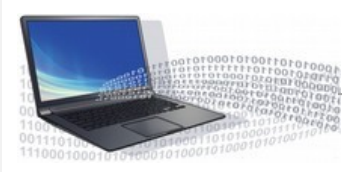
\includegraphics[scale=0.4]{logo.png}
}

\color[RGB]{44,137,4}
\textbf{Сжатие данных}
\color{black}
— процесс, обеспечивающий уменьшение объёма данных путём сокращения их избыточности. \\[0.5em]

Сжатие данных — частный случай кодирования данных. \\[0.5em]

\color[RGB]{44,137,4}
\textbf{Коэффициент сжатия}
\color{black}
— отношение размера входного потока к выходному потоку. \\[0.5em]

\color[RGB]{44,137,4}
\textbf{Отношение сжатия}
\color{black}
— отношение размера выходного потока ко входному потоку. \\[0.5em]

\textbf{Пример.} Размер входного потока равен 500 бит, выходного равен 400 бит. \\
Коэффициент сжатия = 500 бит / 400 бит = 1,25. \\
Отношение сжатия = 400 бит / 500 бит = 0,8. \\[0.5em]

Случайные данные невозможно сжать, так как в них нет никакой избыточности.

\end{frame}

\begin{frame}

\frametitle{
\color[RGB]{153,153,153}
	\begin{flushright}
		\textbf{{\color[RGB]{22,83,126} Т}ипы и методы сжатия данных}\qquad\qquad\qquad
	\end{flushright}
	\hrule
	\vskip -1.5cm\hskip -0.4cm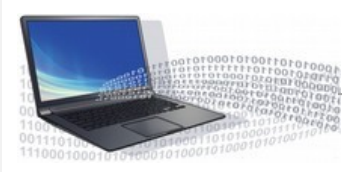
\includegraphics[scale=0.4]{logo.png}
}

\color[RGB]{44,137,4}
\textbf{Сжатие без потерь}
\color{black}
 (полностью обратимое) — сжатые данные после декодирования (распаковки) не отличаются от исходных. \\[0.5em]

\color[RGB]{44,137,4}
\textbf{Сжатие с потерями}
\color{black}
 (частично обратимое) — сжатые данные после декодирования (распаковки) отличаются от исходных, так как при сжатии часть исходных данных была отброшена для увеличения коэффициента cжатия. \\[0.5em]

\color[RGB]{44,137,4}
\textbf{Статистические методы}
\color{black}
— кодирование с помощью усреднения вероятности
появления элементов в закодированной последовательности. \\[0.5em]

\color[RGB]{44,137,4}
\textbf{Словарные методы}
\color{black}
— использование статистической модели данных для разбиения данных на слова с последующей заменой на их индексы в словаре. \\[0.5em]

\end{frame}

\begin{frame}

\frametitle{
\color[RGB]{153,153,153}
	\begin{flushright}
		\textbf{{\color[RGB]{22,83,126} О}шибки при передаче и хранении данных}\qquad\qquad\qquad
	\end{flushright}
	\hrule
	\vskip -1.5cm\hskip -0.4cm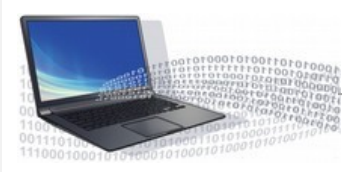
\includegraphics[scale=0.4]{logo.png}
}

Причины: \\
\begin{itemize}
    \item[\textbullet] Альфа-частицы от примесей в чипе микросхемы.
    \item[\textbullet] Нейтроны из фонового космического излучения.
\end{itemize} \\[0.5em]

Частота единичных битовых ошибок (на 1 GB): \\
\begin{itemize}
    \item[\textbullet] От 1 раза в час до 1 раза в тысячелетие (по данным исследования Google получилось ~1 раз в сутки).
\end{itemize}\\[0.5em]

Способы обработки данных:
\begin{itemize}
    \item[\textbullet] Использовать полученные данные без проверки на ошибки.
    \item[\textbullet] Обнаружить ошибку, выполнить запрос повторной передачи поврежденного блока.
    \item[\textbullet] Обнаружить ошибку и отбросить поврежденный блок.
    \item[\textbullet] Обнаружить и исправить ошибку.
    \item[\textbullet] Тройная модульная избыточность.
\end{itemize}

\end{frame}

\end{document}